% !TEX root =./main.tex

\section{Signal $x_8$}

Signal $x_8$ contains an audio signal.  For most of the signal's duration, as can be seen in Figure \ref{fig:x8}, the audio is undisturbed.  However, at about the 8 second mark, narrowband jamming with 3 tones (plus a "tone" at DC) begins.  The tones can be clearly seen in the signal's frequency spectrum in Figure \ref{fig:X8}.  The unfiltered audio can be found in the \code{x8\_unfiltered.wav} file in the \href{https://github.com/dbcometto/ece434_cpx2}{GitHub repository}.

\begin{figure}[H]
    \centering
    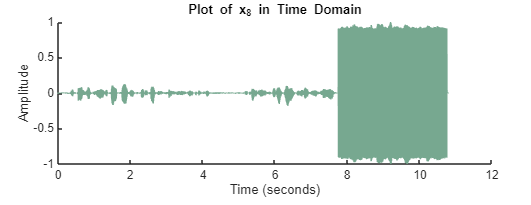
\includegraphics[width=0.5\linewidth]{figures/x8_prefilter.png}
    \caption{Signal $x_8$ over Time}
    \label{fig:x8}
\end{figure}

\begin{figure}[H]
    \centering
    \includegraphics[width=0.5\linewidth]{figures/X8_prefilter.png}
    \caption{Frequency Spectrum of Signal $x_8$}
    \label{fig:X8}
\end{figure}

Focusing on the portion of the frequency spectrum including the tones, it can be seen that the tones are at approximately $1573 \unit{Hz}$, $3151 \unit{Hz}$, and at $4726 \unit{Hz}$ (and at DC).
\begin{figure}[H]
    \centering
    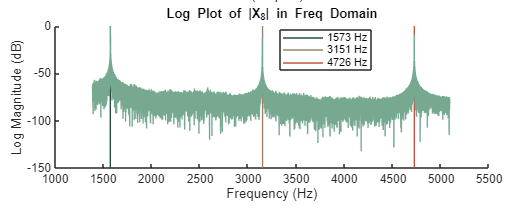
\includegraphics[width=0.5\linewidth]{figures/X8_prefilter_zoom.png}
    \caption{Frequency Spectrum of Signal $x_8$ near Interfering Tones}
    \label{fig:enter-label}
\end{figure}

Up to the 8 second mark, we are able to hear the message, ``He has been eight years upon a project for extracting sunbeams out of cucumbers... He told me, he did not doubt, that, in eight years more---."  The rest of the message (perhaps the secrets for extracting sunbeams from cucumbers?) has been jammed.  In order to recover the message, we must remove the interfering tones.

Again, a notching filter is indicated, as specific frequencies must be stopped.  This notching filter was built by placing poles and zeros.  Because we do not need to preserve linear phase, we can use poles (and thus create an IIR filter).  Converting the tone frequencies to normalized angular frequencies gave the locations of the zeros.  The poles were offset slightly in both angle and magnitude to maximize the notching effect while minimizing the effect on the surrounding frequencies.  For Filter 1, six zeros were used, one for each tone.  The pole zero plot can be seen in Figure \ref{fig:x8_v7_polezero}.

\begin{figure}[H]
    \centering
    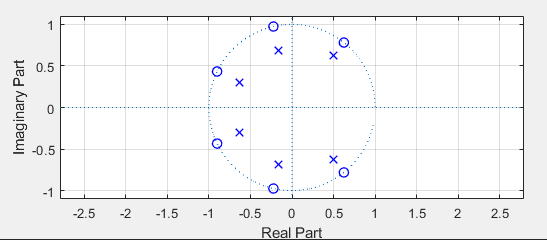
\includegraphics[width=0.5\linewidth]{figures/x8_v7_polezero.png}
    \caption{Pole Zero Plot of Filter 1 for Signal $x_8$}
    \label{fig:x8_v7_polezero}
\end{figure}

The locations of the poles and zeros are compiled in Table \ref{tab:x8_v7}.

\begin{table}[H]
    \centering
    \begin{tabular}{c|cccc}
         Order &      & Zero/Pole & Zero/Pole & Zero/Pole \\ \hline
         6 & Angle    & $\pm 0.8969 \unit{rad}$ & $\pm 1.7962 \unit{rad}$ & $\pm 2.6931 \unit{rad}$ \\
         & Magnitude  & $1$/$0.8$ & $1$/$0.8$ & $1$/$0.8$ 
    \end{tabular}
    \caption{Parameters for Filter 1 for Signal $x_8$}
    \label{tab:x8_v7}
\end{table}


Applying this filter to the signal results in the removal of the majority of the interference.  However, the tones are still present, albeit at a diminished volume.  The signal response can be seen in Figure \ref{fig:x8_v7_response}.  The audio information is clearly able to be heard, as can be verified in the \code{x8\_filter7.wav} file in the \href{https://github.com/dbcometto/ece434_cpx2}{GitHub repository}.
\begin{figure}[H]
    \centering
    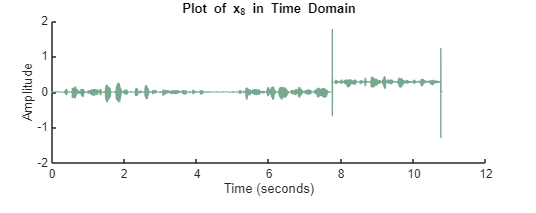
\includegraphics[width=0.5\linewidth]{figures/x8_filterv7.png}
    \includegraphics[width=0.5\linewidth]{figures/X8_filterv7.png}
    \caption{Response of Signal $x_8$ to Filter 1, Order 6}
    \label{fig:x8_v7_response}
\end{figure}

To fully remove the tones, the filter can be modified to order 12, placing two zeros at each tone's frequency.  This change results in Filter 2.  The pole zero plot for Filter 2 can be seen in Figure \ref{fig:x8_v5_polezero}.

\begin{figure}[H]
    \centering
    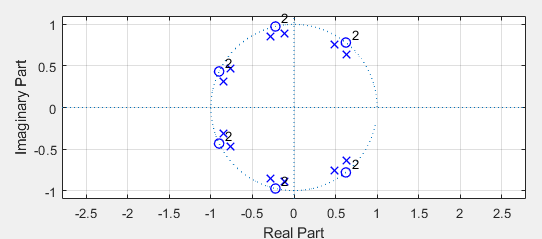
\includegraphics[width=0.5\linewidth]{figures/x8_v5_polezero.png}
    \caption{Pole Zero Plot of Filter 2 for Signal $x_8$}
    \label{fig:x8_v5_polezero}
\end{figure}

The locations of the zeros are the same as in Filter 1.  The poles' magnitude were increased to $0.9$, and they are placed $\pm 0.1 \unit{rad}$ from the angle of their corresponding zero.

The signal response to Filter 2 can be seen in Figure \ref{fig:x8_v5_response}.  Now, the tones have been completely removed, but there is a DC shift and two pops can be heard during the jammed portion of the signal.  The output audio can be heard in the \code{x8\_filter12.wav} file in the \href{https://github.com/dbcometto/ece434_cpx2}{GitHub repository}.  It is not necessary to remove these artifacts, as they do not interfere with the content of the signal.

\begin{figure}[H]
    \centering
    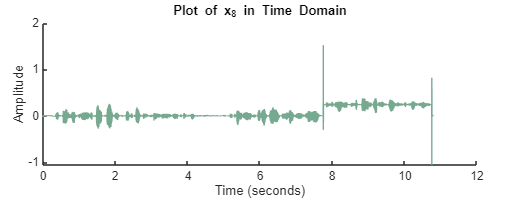
\includegraphics[width=0.5\linewidth]{figures/x8_filterv5.png}
    \includegraphics[width=0.5\linewidth]{figures/X8_filterv5.png}
    \caption{Response of Signal $x_8$ to Filter 2, order 12}
    \label{fig:x8_v5_response}
\end{figure}

However, in order to maximally enhance the audio and remove these final artifacts, zeros and corresponding poles are added near DC, resulting in Filter 3.  The response to Filter 3 can be seen in Figure \ref{fig:x8_14}

\begin{figure}[H]
    \centering
    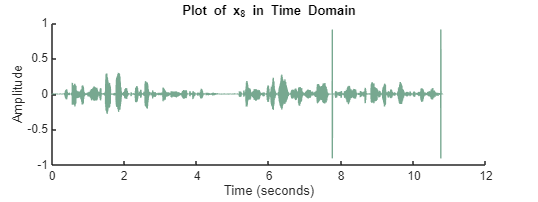
\includegraphics[width=0.5\linewidth]{figures/x8_filter11.png}
    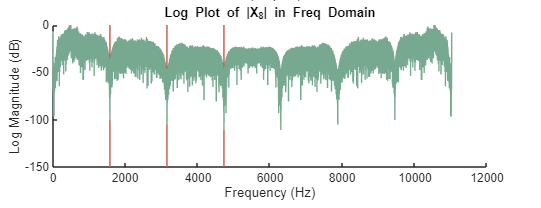
\includegraphics[width=0.5\linewidth]{figures/X8_filterv11.png}
    \caption{Response of Signal $x_8$ to Filter 3}
    \label{fig:x8_14}
\end{figure}

Additionally, the pops are manually removed from the audio by setting the corresponding portions of the time signal to zero.  A final, completely clean output can be seen in Figure \ref{fig:x8_clean}, and heard in the \code{x8\_filterNoPop.wav} file in the \href{https://github.com/dbcometto/ece434_cpx2}{GitHub repository}.

\begin{figure}[H]
    \centering
    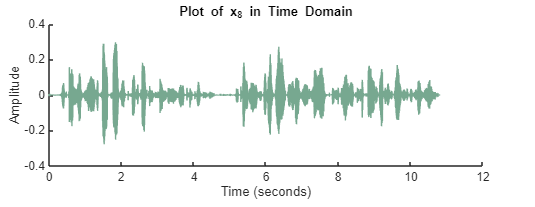
\includegraphics[width=0.5\linewidth]{figures/x8_nopops.png}
    \caption{Signal $x_8$ after Filter 3 and Editing}
    \label{fig:x8_clean}
\end{figure}

As can be heard following the application of any of the 3 filters, the complete message is, ``He has been eight years upon a project for extracting sunbeams out of cucumbers... He told me, he did not doubt, that, in eight years more, he should be able to supply the governor’s gardens with sunshine."  Originally, I misheard several of the words.  However, a Google search revealed that it is an abridged quote from \textit{Gulliver's Travels}, which enabled me to correct the words that I heard incorrectly.